% !TEX root = task-2-9-1.tex
% Editable task bank. Append new BankTask blocks at the end of the document.
\documentclass[12pt,a4paper]{article}
\usepackage{physics-textbook}
\usepackage{graphicx,needspace}
\usetikzlibrary{decorations.pathmorphing}
\newif\ifShowSolutions
\ifdefined\TutorEdition
  \ShowSolutionstrue
\else
  \ShowSolutionsfalse % Change to \ShowSolutionstrue to display solutions.
\fi
\newcounter{banktask}
\newsavebox{\BankTaskBox}
\newcommand{\BankTaskContent}[3]{%
  \noindent\textbf{\thebanktask.}\quad #2\par
  \ifShowSolutions
    \Needspace{50mm}% Keep the solution heading with its opening text or diagram.
    #3\par
    \ifdefined\TutorEdition
      \ifcsname TutorSource#1\endcsname
        \nopagebreak\smallskip{\small\csname TutorSource#1\endcsname\par}%
      \fi
    \fi
  \fi
}
\newcommand{\BankTask}[3]{%
  \refstepcounter{banktask}\par\medskip
  \sbox{\BankTaskBox}{\begin{minipage}{\linewidth}%
    \BankTaskContent{#1}{#2}{#3}\end{minipage}}%
  \ifdim\dimexpr\ht\BankTaskBox+\dp\BankTaskBox\relax>\dimexpr\textheight-20mm\relax
    \Needspace{35mm}\BankTaskContent{#1}{#2}{#3}%
  \else
    \Needspace{\dimexpr\ht\BankTaskBox+\dp\BankTaskBox\relax}%
    \noindent\usebox{\BankTaskBox}\par
  \fi
  \medskip
}
\begin{document}
\BookSubsection{2.9.1}{Удельная теплоёмкость}


% Source sdamgia-1004: https://phys-ege.sdamgia.ru/problem?id=1004
\BankTask{sdamgia-1004}{
Температура медного образца массой $100\,\text{г}$ повысилась с $20^\circ\text{C}$ до $60^\circ\text{C}$. Какое количество теплоты получил образец? (В джоулях.) Удельную теплоемкость меди считать равной $380\text{Дж}/ ( \text{кг} \cdot ^\circ\text{C} ) .$
}{
\smallskip\noindent\textbf{Решение}\par
На нагрев $m=0{,}1\text{кг}$ меди, удельная теплоемкость которой $c=380\text{Дж}/ ( \text{кг} \cdot ^\circ\text{C} ) ,$ от температуры $t_1=20 ^\circ\text{C}$ до температуры $t_2=60 ^\circ\text{C}$ необходимо затратить количество теплоты:

$Q=cm ( t_2 - t_1 ) =380 \cdot 0{,}1 \cdot ( 60 - 20 ) \text{Дж}=1520\text{Дж}.$

Ответ: $1520$.
}

% Source sdamgia-1109: https://phys-ege.sdamgia.ru/problem?id=1109
\BankTask{sdamgia-1109}{
Чтобы нагреть $96\,\text{г}$ молибдена на $1\,\text{К}$, нужно передать ему количество теплоты равное $24\,\text{Дж}$. Чему равна удельная теплоемкость этого вещества? (В джоулях на килограмм на Кельвин.)
}{
\smallskip\noindent\textbf{Решение}\par
На нагрев $m=0{,}096\text{кг}$ молибдена на $1\text{К}$ необходимо затратить количество теплоты $Q=cm \cdot \Delta T=24\text{Дж}.$ Отсюда находим удельную теплоемкость молибдена:

$c= \frac{Q}{m \cdot \Delta T} = \frac{24}{0{,}096 \cdot 1} \text{Дж}/ ( \text{кг} \cdot K ) =250\text{Дж}/ ( \text{кг} \cdot K ) .$

Ответ: $250$.
}

% Source sdamgia-6231: https://phys-ege.sdamgia.ru/problem?id=6231
\BankTask{sdamgia-6231}{
Алюминиевому и железному цилиндрам одинаковой массы сообщили одинаковое количество теплоты. Определите примерное отношение изменения температур этих цилиндров $\frac{\Delta t_{\mathrm{Al}}}{\Delta t_{\mathrm{Fe}}} .$ Удельная теплоемкость железа равна $460\,\text{Дж}/(\text{кг}\cdot\text{К})$, алюминия — $900\,\text{Дж}/(\text{кг}\cdot\text{К})$. (До десятых.)
}{
\smallskip\noindent\textbf{Решение}\par
При нагревании тела на температуру $\Delta t$ ему передается количество теплоты $Q=mc\Delta t.$ Тела получили одинаковое количество теплоты, то есть $Q_{\mathrm{Fe}}=Q_{\mathrm{Al}}.$ Имеем:

$Q_{\mathrm{Fe}}=Q_{\mathrm{Al}} \Longleftrightarrow m_{\mathrm{Fe}}c_{\mathrm{Fe}}\Delta t_{\mathrm{Fe}}=m_{\mathrm{Al}}c_{\mathrm{Al}}\Delta t_{\mathrm{Al}} \Longleftrightarrow \frac{\Delta t_{\mathrm{Al}}}{\Delta t_{\mathrm{Fe}}} = \frac{c_{\mathrm{Fe}}}{c_{\mathrm{Al}}} = \frac{460}{900} \approx0{,}5.$

Ответ: $0{,}5$.
}

% Source sdamgia-1003: https://phys-ege.sdamgia.ru/problem?id=1003
\BankTask{sdamgia-1003}{
\begin{center}\begin{tikzpicture}[task graph]
\draw[task grid,step=1] (0,0) grid (4,3);\draw[task axis,->](0,0)--(4.3,0)node[right]{$Q,\,\text{кДж}$};\draw[task axis,->](0,0)--(0,3.3)node[above left]{$T,\,\text{К}$};\node[below left]at(0,0){$0$};\foreach\y/\s in{0/200,1/300,2/400}{\node[left]at(0,\y){$\s$};}\foreach\x/\s in{1/100,2/200}{\fill(\x,0)circle(1.5pt);\node[below]at(\x,0){$\s$};}\fill(0,1)circle(1.5pt)(0,2)circle(1.5pt);\draw[task curve](0,2)--(2,1);
\end{tikzpicture}\end{center}
На рисунке приведен график зависимости температуры твердого тела от отданного им количества теплоты. Масса тела $4\,\text{кг}$. Какова удельная теплоемкость вещества этого тела? (В джоулях на килограмм на кельвин.)
}{
\smallskip\noindent\textbf{Решение}\par
Из графика видно, что, отдав $Q=200\text{кДж}$ тело охладилось на $\Delta T=400\text{К} - 300\text{К}=100\text{К}.$ Следовательно, удельная теплоемкость вещества этого тела равна:

$c= \frac{Q}{m\Delta T} = \frac{200\text{кДж}}{4\text{кг} \cdot 100\text{К}} = \frac{200 \cdot 10 ^{3} \text{Дж}}{4\text{кг} \cdot 100\text{К}} =500\text{Дж}/ ( \text{кг} \cdot \text{К} ) .$

Ответ: $500$.
}

% Source sdamgia-25242: https://phys-ege.sdamgia.ru/problem?id=25242
\BankTask{sdamgia-25242}{
В медный калориметр массой $500\,\text{г}$, находившийся при температуре $20^\circ\text{C}$, налили $200\,\text{г}$ воды, температура которой была равна $50^\circ\text{C}$. Через некоторое время, когда между водой и калориметром установилось тепловое равновесие, температура воды в нем оказалась равной $40^\circ\text{C}$. Какое количество теплоты было отдано водой и калориметром в окружающую среду? (В джоулях.)
}{
\smallskip\noindent\textbf{Решение}\par
Теплота, полученная калориметром, равна $Q_1=m_1c_1 ( t - t_1 ) =0{,}5 \cdot 380 \cdot ( 40 - 20 ) =3800\text{Дж}.$

Теплота, отданная водой, равна $Q_2=m_2c_2 ( t - t_2 ) =0{,}2 \cdot 4200 \cdot ( 40 - 50 ) = - 8400\text{Дж}.$

Теплота, отданная в окружающую среду, равна $Q=|Q_2| - Q_1=8400 - 3800=4600\text{Дж}.$

Ответ: $4600$.
}

% Source sdamgia-10956: https://phys-ege.sdamgia.ru/problem?id=10956
\BankTask{sdamgia-10956}{
При выполнении лабораторной работы по физике ученики должны были экспериментально определить удельную теплоемкость вещества, из которого изготовлено некоторое тело. Данное тело сначала помещали в калориметр с холодной водой и дожидались установления теплового равновесия. Затем тело погружали в другой калориметр — с горячей водой — и также дожидались установления теплового равновесия. В ходе работы проводились необходимые измерения, пользуясь результатами которых, в дальнейшем можно было определить удельную теплоемкость вещества.

Для выполнения этой лабораторной работы ученикам было выдано следующее оборудование: два пустых калориметра, сосуды с холодной и горячей водой, исследуемое тело на нити, мензурку.

Какие два предмета из приведенного ниже перечня оборудования необходимо дополнительно использовать для проведения этого эксперимента, если теплоемкостью калориметров экспериментаторы решили пренебречь и удельная теплоемкость воды считается известной?

$1$. Термометр.

$2$. Часы.

$3$. Электронные весы.

$4$. Линейку.

$5$. Штатив.
}{
\smallskip\noindent\textbf{Решение}\par
Для определения удельной теплоемкости тела необходимо знать массу тела и воды, а также температуру воды в начале и конце процесса передачи тепла.

Ответ: $13$.
}

% Source sdamgia-35142: https://phys-ege.sdamgia.ru/problem?id=35142
\BankTask{sdamgia-35142}{
В калориметр со льдом, имеющим температуру $0^\circ\text{C}$, добавили воду при комнатной температуре. Как изменится в результате установления теплового равновесия следующие величины: удельная теплоемкость воды, масса льда?

$1$. Увеличивается.

$2$. Уменьшается.

$3$. Не изменяется.

\begin{center}\begin{tabular}{|p{0.43\linewidth}|p{0.43\linewidth}|}\hline
Удельная теплоемкость воды & Масса льда\\\hline
\strut & \strut\\\hline\end{tabular}\end{center}
}{
\smallskip\noindent\textbf{Решение}\par
Удельная теплоемкость воды не зависит от изменения температуры, массы и количества отданной теплоты. Эта величина не изменится ($3$).

В результате теплообмена лед будет получать теплоту от воды и плавиться, следовательно, его масса уменьшится ($2$).

Ответ: $32$.
}

% Source sdamgia-3757: https://phys-ege.sdamgia.ru/problem?id=3757
\BankTask{sdamgia-3757}{
Высота непрерывного падения воды самого высокого в мире водопада Анхель — $807$ метров. На сколько градусов могла бы повыситься температура падающей воды, если считать, что на ее нагревание затрачивается $50$\% работы, совершаемой силой тяжести?
}{
\smallskip\noindent\textbf{Решение}\par
Определим какую работу совершает сила тяжести при переносе воды массой $m$ с высоты водопада Анхель: $A_{\text{тяж}}=mgh.$ Для нагрева воды массой $m$ на температуру $\Delta T$ необходимо затратить энергию $Q=cm\Delta T.$ Составим уравнение теплового баланса, учитывая, что только $50$\% работы силы тяжести идет на нагрев воды: 

$Q= \frac{A_{\text{тяж}}}{2} ,$ откуда $cm\Delta T= \frac{mgh}{2}$

 Отсюда изменение температуры жидкости равно: 

$\Delta T= \frac{gh}{2c} = \frac{10\text{м}/\text{с} ^{2} \cdot 807\text{м}}{2 \cdot 4200\text{Дж}/ ( \text{кг} \cdot \text{К} )} \approx 0{,}96\text{К}.$

Ответ: $0{,}96\,\text{К}$.
}

% Source sdamgia-7059: https://phys-ege.sdamgia.ru/problem?id=7059
\BankTask{sdamgia-7059}{
Препарат с активностью $1{,}7\cdot 10^{11}$ частиц в секунду помещен в металлический контейнер массой $0{,}5\,\text{кг}$. За $2\,\text{ч}$ температура контейнера повысилась на $5{,}2^\circ\text{C}$. Известно, что данный препарат испускает $\alpha$-частицы с энергией $5{,}3\,\text{МэВ}$, причем практически вся энергия $\alpha$-частиц переходит во внутреннюю энергию контейнера. Найдите удельную теплоемкость металла контейнера. Теплоемкостью препарата и теплообменом с окружающей средой пренебречь.

(В единицах СИ; до целого числа.)
}{
\smallskip\noindent\textbf{Решение}\par
За время $\Delta t$ в препарате выделяется количество теплоты $Q=AE \Delta t.$ Изменение температуры контейнера определяется равенством $Q=c m \Delta T.$ Выделившееся количество теплоты идет на нагревание контейнера. Отсюда:

$c= \frac{AE \Delta t}{m\Delta T} = \frac{1{,}7 \cdot 10 ^{11} \cdot 5{,}3 \cdot 1{,}6 \cdot 10 ^{- 13} \cdot 7200}{0{,}5 \cdot 5{,}2} \approx 399 \text{Дж}/ ( \text{кг} \cdot ^\circ\text{C} ) .$

Ответ: $399 \text{Дж}/ ( \text{кг} \cdot \! ^\circ\text{C} ) .$
}

% Source sdamgia-19745: https://phys-ege.sdamgia.ru/problem?id=19745
\BankTask{sdamgia-19745}{
На заводе изготовили биметаллическую деталь в виде сплошного цилиндра, внутренняя осесимметричная цилиндрическая часть которого выполнена из железа, а остальная — из алюминия. Площадь поперечного сечения алюминиевой части цилиндра в $2$ раза больше, чем у железной, а масса всей детали равна $m=1{,}5\,\text{кг}$. Какое количество теплоты нужно сообщить этой детали для того, чтобы повысить ее температуру на $1\,\text{К}$?
}{
\smallskip\noindent\textbf{Решение}\par
$1$. Обозначим длину цилиндра $l$, площадь сечения железной части детали $S$, тогда алюминиевая часть по условию будет иметь площадь сечения $2S$. Плотности железа и алюминия $\rho_{\text{ж}}$ и $\rho_{\text{ал}}$ приведены в таблицах, как и удельные теплоемкости этих металлов $c_{\text{ж}}$ и $c_{\text{ал}}.$

$2$. Исходя из формулы для связи массы с плотностью и объемом тел, можно записать для массы всей детали, состоящей из двух частей: $m = \rho_{\text{ж}}Sl + 2\rho_{\text{ал}}Sl.$ Отсюда объем железа равен $Sl = \frac{m}{\rho_{\text{ж}} + 2\rho_{\text{ал}}} ,$ его масса равна $m_{\text{ж}} = m\rho_{\text{ж}}/ ( \rho_{\text{ж}} + 2\rho_{\text{ал}} ) ,$ и аналогичным образом получаем, что масса алюминия равна $m_{\text{ал}} = \frac{2m\rho_{\text{ал}}}{\rho_{\text{ж}} + 2\rho_{\text{ал}}} .$

$3$. Для того чтобы повысить температуру этой детали на $\Delta T = 1\text{К},$ необходимо сообщить ей количество теплоты 

$Q = c_{\text{ж}}m_{\text{ж}}\Delta T + c_{\text{ал}}m_{\text{ал}}\Delta T = \frac{m\Delta T ( c_{\text{ж}}\rho_{\text{ж}} + 2c_{\text{ал}}\rho_{\text{ал}} )}{\rho_{\text{ж}} + 2\rho_{\text{ал}}} .$

Подставляя численные значения, получаем:

$Q = \frac{1{,}5 \text{кг} \cdot 1 \text{К} \cdot ( 460 \text{Дж}/ ( \text{кг} \cdot \! ^\circ\text{C} ) \cdot 7800\text{кг}/\text{м} ^{3} + 2 \cdot 900\text{Дж}/ ( \text{кг} \cdot \! ^\circ\text{C} ) \cdot 2700\text{кг}/\text{м} ^{3} )}{7800 \text{кг}/\text{м} ^{3} + 2 \cdot 2700\text{кг}/\text{м} ^{3}} = 960\text{Дж}.$

Ответ: $Q = 960\text{Дж}.$
}


% Source F45AFF: https://ege.fipi.ru/bank/questions.php?search=1&proj=BA1F39653304A5B041B656915DC36B38&qid=F45AFF
\BankTask{F45AFF}{
\begin{center}
\begin{tikzpicture}[task graph,x=1cm,y=1cm]
\draw[task axis] (0,0)--(4.5,0) node[below] {$Q,\,\text{кДж}$};
\draw (0,0)--(0,0.44);
\draw[task axis] (0,0.68)--(0,3.35) node[left] {$T,\,\text{К}$};
\draw (-0.09,0.46)--(0.02,0.52)--(0.12,0.48);
\draw (-0.09,0.57)--(0.02,0.63)--(0.12,0.59);
\node[below left] at (0,0) {$0$};
\draw (0.42,-0.06)--(0.48,0.06);\draw (0.54,-0.06)--(0.60,0.06);
\draw[task projection] (1.45,0)--(1.45,1.05);
\draw[task projection] (3.1,0)--(3.1,2.6);
\node[below] at (1.45,0) {$100$};
\node[below] at (3.1,0) {$136$};
\draw[task projection] (0,1.05)--(1.45,1.05);
\draw[task projection] (0,2.6)--(3.1,2.6);
\node[left] at (0,1.05) {$273$};
\node[left] at (0,2.6) {$293$};
\draw[task curve] (0.7,0.3454545)--(3.1,2.6);
\fill (1.45,1.05) circle (1.7pt);
\fill (3.1,2.6) circle (1.7pt);
\end{tikzpicture}
\end{center}
На рисунке показана зависимость температуры металлической детали массой $2\,\text{кг}$ от переданного ей количества теплоты. Чему равна удельная теплоёмкость металла (в $\text{Дж}/(\text{кг}\cdot\text{К})$)?
}{
\smallskip\noindent\textbf{Решение от GPT}\par
Используем $\Delta Q=mc\Delta T$. По графику $\Delta Q=(136-100)\,\text{кДж}=36000\,\text{Дж}$, $\Delta T=293-273=20\,\text{К}$. Тогда
\[
c=\frac{\Delta Q}{m\Delta T}=\frac{36000}{2\cdot20}=900\,\frac{\text{Дж}}{\text{кг}\cdot\text{К}}.
\]
Ответ: $900$.
}

% Source 687697: https://ege.fipi.ru/bank/questions.php?search=1&proj=BA1F39653304A5B041B656915DC36B38&qid=687697
\BankTask{687697}{
На сколько градусов нагреются \(100\,\text{г}\) свинца, если ему сообщить \(260\,\text{Дж}\) теплоты (в ${}^\circ\text{C}$)?
}{
\smallskip\noindent\textbf{Решение от GPT}\par
Используем табличную удельную теплоёмкость свинца \(c=130\,\text{Дж}/(\text{кг}\cdot\text{К})\). При \(m=0{,}1\,\text{кг}\)
\[
\Delta T=\frac{Q}{cm}=\frac{260}{130\cdot0{,}1}=20\,\text{К}.
\]
Ответ: \(20\,{}^\circ\text{C}\).
}

% Source 772CBF: https://ege.fipi.ru/bank/questions.php?search=1&proj=BA1F39653304A5B041B656915DC36B38&qid=772CBF
\BankTask{772CBF}{
Температура куска металла с удельной теплоёмкостью $900\,\text{Дж}/(\text{кг}\cdot\text{К})$ понизилась со $120\,{}^\circ\text{C}$ до $40\,{}^\circ\text{C}$. При этом выделилось количество теплоты, равное $108\,\text{кДж}$. Чему равна масса этого куска металла (в $\text{кг}$)?
}{
\smallskip\noindent\textbf{Решение от GPT}\par
$Q=cm(t_1-t_2)$, откуда $m=Q/[c(t_1-t_2)]=108000/(900\cdot80)=1{,}5\,\text{кг}$. Ответ: $1{,}5\,\text{кг}$.
}

% Source 35852E: https://ege.fipi.ru/bank/questions.php?search=1&proj=BA1F39653304A5B041B656915DC36B38&qid=35852E
\BankTask{35852E}{
Горячее вещество, первоначально находившееся в жидком состоянии, медленно охлаждали. Мощность теплоотвода постоянна. В таблице приведены результаты измерений температуры вещества с течением времени.
\begin{center}
\begin{tabular}{|l|r|r|r|r|r|r|r|r|}
\hline
Время, $\text{мин}$ & \(0\) & \(5\) & \(10\) & \(15\) & \(20\) & \(25\) & \(30\) & \(35\) \\
\hline
Температура, \({}^{\circ}\mathrm{C}\) & \(250\) & \(242\) & \(234\) & \(232\) & \(232\) & \(232\) & \(230\) & \(216\) \\
\hline
\end{tabular}
\end{center}
\begin{enumerate}
\item Температура плавления вещества в данных условиях равна \(232\,{}^{\circ}\mathrm{C}\).
\item Через \(20\,\text{мин}\). после начала измерений вещество находилось только в твёрдом состоянии.
\item Удельная теплоёмкость вещества в жидком и твёрдом состояниях одинакова.
\item Через \(30\,\text{мин}\). после начала измерений вещество находилось только в твёрдом состоянии.
\item Процесс кристаллизации вещества занял более \(25\,\text{мин}\).
\end{enumerate}
}{
\smallskip\noindent\textbf{Решение от GPT}\par
\begin{enumerate}
\item Верно: участок постоянной температуры соответствует кристаллизации, поэтому \(T_{\text{пл}}=232\,{}^{\circ}\mathrm{C}\).
\item Неверно: в момент \(t=20\,\text{мин}\) идёт кристаллизация, присутствуют жидкая и твёрдая фазы.
\item Неверно: при постоянной мощности \(P=mc\lvert\Delta T/\Delta t\rvert\). Скорости охлаждения жидкости и твёрдого вещества равны соответственно \(8/5=1{,}6\) и \(14/5=2{,}8\,{}^{\circ}\mathrm{C}/\text{мин}\); теплоёмкости различны.
\item Верно: через \(30\,\text{мин}\) температура \(230\,{}^{\circ}\mathrm{C}\) ниже температуры кристаллизации, вещество полностью затвердело.
\item Неверно: кристаллизация началась после \(10\,\text{мин}\) и завершилась до \(30\,\text{мин}\), поэтому её длительность меньше \(20\,\text{мин}\).
\end{enumerate}
Ответ: \(14\).
}

% Source F72E75: https://ege.fipi.ru/bank/questions.php?search=1&proj=BA1F39653304A5B041B656915DC36B38&qid=F72E75
\BankTask{F72E75}{
На рисунке представлены графики зависимости температуры \(t\) двух тел одинаковой массой от сообщённого им количества теплоты \(Q\). Каждое тело находится в сосуде под поршнем. Первоначально тела находились в жидком агрегатном состоянии.
\begin{center}
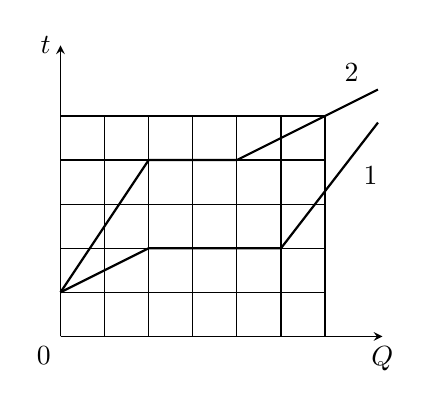
\begin{tikzpicture}[>=stealth,x=0.56cm,y=0.56cm]
\draw[step=1,thin] (0,0) grid (6,5);
\draw[->] (0,0)--(7.3,0) node[below] {$Q$};
\draw[->] (0,0)--(0,6.6) node[left] {$t$};
\node[below left] at (0,0) {$0$};
\draw[thick] (0,1)--(2,2)--(5,2)--(7.2,4.85);
\draw[thick] (0,1)--(2,4)--(4,4)--(7.2,5.6);
\node[right] at (6.65,3.65) {$1$};
\node[above] at (6.6,5.55) {$2$};
\end{tikzpicture}
\end{center}
\begin{enumerate}
\item Температура кипения первого тела в \(2\) раза меньше, чем температура кипения второго тела.
\item Тела имеют одинаковую удельную теплоёмкость в газообразном состоянии.
\item Удельная теплоёмкость в жидком агрегатном состоянии у второго тела в \(3\) раза меньше, чем у первого.
\item Оба тела имеют одинаковую удельную теплоту парообразования.
\item Для первого тела удельная теплоёмкость в жидком агрегатном состоянии меньше удельной теплоёмкости в газообразном состоянии.
\end{enumerate}
}{
\smallskip\noindent\textbf{Решение от GPT}\par
При нагревании \(c=\Delta Q/(m\Delta t)\), при кипении \(L=\Delta Q/m\). Массы одинаковы.
\begin{enumerate}
\item Верно: горизонтальные участки расположены на уровнях \(2\) и \(4\) клеток от нуля температуры, поэтому \(t_{\text{кип},1}=t_{\text{кип},2}/2\).
\item Неверно: наклоны участков нагревания пара различаются, следовательно, теплоёмкости различны.
\item Верно: при одинаковом количестве теплоты на начальных участках \(\Delta t_1=1\) клетка, \(\Delta t_2=3\) клетки. Поэтому \(c_2=c_1/3\).
\item Неверно: длины участков кипения равны \(3\) и \(2\) клеткам по оси \(Q\), поэтому \(L_1/L_2=3/2\).
\item Неверно: участок нагревания пара первого тела круче участка нагревания жидкости, поэтому \(c_{\text{газ},1}<c_{\text{ж},1}\).
\end{enumerate}
\(\boxed{13}\).
}

% Source A53641: https://ege.fipi.ru/bank/questions.php?search=1&proj=BA1F39653304A5B041B656915DC36B38&qid=A53641
\BankTask{A53641}{
\begin{center}
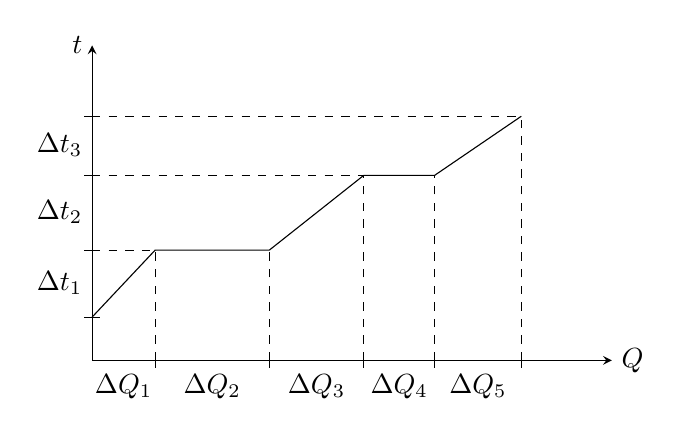
\begin{tikzpicture}[x=1cm,y=1cm,>=stealth]
\draw[->] (0,0)--(6.6,0) node[right] {$Q$};
\draw[->] (0,0)--(0,4) node[left] {$t$};
\draw (0,0.55)--(0.8,1.4)--(2.25,1.4)--(3.45,2.35)--(4.35,2.35)--(5.45,3.1);
\foreach \x/\y in {0.8/1.4,2.25/1.4,3.45/2.35,4.35/2.35,5.45/3.1} {
\draw[dashed] (\x,0)--(\x,\y);
\draw (\x,0.1)--(\x,-0.1);
}
\foreach \y in {0.55,1.4,2.35,3.1} {\draw (-0.1,\y)--(0.1,\y);}
\draw[dashed] (0,1.4)--(0.8,1.4);
\draw[dashed] (0,2.35)--(3.45,2.35);
\draw[dashed] (0,3.1)--(5.45,3.1);
\node[left] at (0,0.98) {$\Delta t_1$};
\node[left] at (0,1.88) {$\Delta t_2$};
\node[left] at (0,2.73) {$\Delta t_3$};
\node[below] at (0.4,-0.06) {$\Delta Q_1$};
\node[below] at (1.525,-0.06) {$\Delta Q_2$};
\node[below] at (2.85,-0.06) {$\Delta Q_3$};
\node[below] at (3.9,-0.06) {$\Delta Q_4$};
\node[below] at (4.9,-0.06) {$\Delta Q_5$};
\end{tikzpicture}
\end{center}
В цилиндре под поршнем находилось твёрдое вещество массой $m$. Цилиндр поместили в печь. На рисунке схематично показан график изменения температуры $t$ вещества по мере поглощения им количества теплоты $Q$. Формулы А и Б позволяют рассчитать значения физических величин, характеризующих происходящие с веществом тепловые процессы.

Установите соответствие между формулами и физическими величинами, значение которых можно рассчитать по этим формулам.



\begin{center}
\TaskMatchingColumns[.35\linewidth]{Формулы}{
А) $\displaystyle\frac{\Delta Q_1}{m\Delta t_1}$\par
Б) $\displaystyle\frac{\Delta Q_2}{m}$
}{Физические величины}{
1) удельная теплота плавления\par
2) удельная теплота парообразования\par
3) удельная теплоёмкость твёрдого вещества\par
4) удельная теплоёмкость жидкости
}

\begin{tabular}{|c|c|}
\hline
А & Б \\
\hline
\phantom{3} & \phantom{1} \\
\hline
\end{tabular}
\end{center}
}{
\smallskip\noindent\textbf{Решение от GPT}\par
А: первый наклонный участок соответствует нагреванию твёрдого вещества. Из $\Delta Q_1=mc_{\text{тв}}\Delta t_1$ получаем $c_{\text{тв}}=\dfrac{\Delta Q_1}{m\Delta t_1}$, поэтому А~--- 3.

Б: первый горизонтальный участок соответствует плавлению при постоянной температуре. Из $\Delta Q_2=\lambda m$ получаем $\lambda=\dfrac{\Delta Q_2}{m}$, поэтому Б~--- 1.

Ответ: $31$.
}

% Source 3283: https://phys-ege.sdamgia.ru/problem?id=3283
\BankTask{3283}{
Железному и алюминиевому цилиндрам сообщили одинаковое количество теплоты, что привело к одинаковым изменениям температуры цилиндров. Воспользовавшись таблицами, приведенными в справочнике, определите примерное отношение масс этих цилиндров $\frac{m_{Fe}}{m_{Al}} .$
}{
\smallskip\noindent\textbf{Решение}\par
Количество теплоты, необходимое для нагревания тела массой m на температуру $\Delta t,$ дается выражением $Q=cm\Delta t.$  По условию, $Q_{Fe}=Q_{Al},\Delta t_{Fe}=\Delta t_{Al},$ а значит:

\[\frac{m_{Fe}}{m_{Al}} = \frac{c_{Al}}{c_{Fe}} = \frac{900\,\text{Дж/кг} \cdot K}{460\,\text{Дж/кг} \cdot K} \approx 2.\]

Ответ: $2$.
}

\end{document}
